\documentclass[a4paper,12pt]{article}

\textwidth 17cm \textheight 25cm \evensidemargin 0cm
\oddsidemargin 0cm \topmargin -2cm
\parindent 0pt
%\parskip \bigskipamount

\usepackage{graphicx}
\usepackage[dutch]{babel}
\usepackage{amssymb,amsthm,amsmath}
%\usepackage{dot2texi}
\usepackage[utf8]{inputenc}
\usepackage{nopageno}
\usepackage{pdfpages}
\usepackage{enumerate}
\usepackage{caption}
\usepackage{wrapfig}
\usepackage{pgf,tikz,pgfplots}
\pgfplotsset{compat=1.15}
\usepackage{color}
\usetikzlibrary{arrows}
\usetikzlibrary{patterns}
\usepackage{fancyhdr}
\pagestyle{fancy}
\usepackage[version=3]{mhchem}
\usepackage{multicol}
\usepackage{fix-cm}
\usepackage{setspace}
\usepackage{mhchem}
\usepackage{xhfill}
\usepackage{parskip}
\usepackage{cancel}
\usepackage{mdframed}
\usepackage{url}
\usepackage{mathtools}
\usepackage{changepage}

\newcommand{\todo}[1]{{\color{red} TODO: #1}}

\newcommand{\degree}{\ensuremath{^\circ}}
\newcommand\rad{\qopname\relax o{\mathrm{rad}}}

\newcommand\ggd{\qopname\relax o{\mathrm{ggd}}}

\pgfmathdeclarefunction{gauss}{2}{%
  \pgfmathparse{1/(#2*sqrt(2*pi))*exp(-((x-#1)^2)/(2*#2^2))}%
}

\def\LRA{\Leftrightarrow}

\newcommand{\zrmbox}{\framebox{\phantom{EXE}}\phantom{X}}
\newcommand{\zrm}[1]{\framebox{#1}}

% environment oefening:
% houdt een teller bij die de oefeningen nummert, probeert ook de oefening op één pagina te houden
\newcounter{noefening}
\setcounter{noefening}{0}
\newenvironment{oefening}
{
  \stepcounter{noefening}
  \pagebreak[0]
  \begin{minipage}{\textwidth}
  \vspace*{0.7cm}{\large\bf Oefening \arabic{noefening}}
}{%
  \end{minipage}
}

\usepackage{calc}

% vraag
\reversemarginpar
\newcounter{punten}
\setcounter{punten}{0}
\newcounter{nvraag}
\setcounter{nvraag}{1}
\newlength{\puntwidth}
\newlength{\boxwidth}
\newcommand{\vraag}[1]{
\settowidth{\puntwidth}{\Large{#1}}
\setlength{\boxwidth}{1.5cm}
\addtolength{\boxwidth}{-\puntwidth}
{\large\bf Vraag \arabic{nvraag} \addtocounter{nvraag}{1}}\vspace*{-0.5cm}
{\marginpar{\color{lightgray}\fbox{\parbox{1.5cm}{\vspace*{1cm}\hspace*{\boxwidth}{\Large{#1}}}}}
\vspace*{0.5cm}}
\addtocounter{punten}{#1}}

% arulefill
\def\arulefill{\leavevmode{\xrfill[-5pt]{0.3pt}[lightgray]\endgraf}\vspace*{0.2cm}}

% \arules{n}
\newcommand{\arules}[1]{
\color{lightgray}
%\vspace*{0.05cm}
\foreach \n in {1,...,#1}{
  \vspace*{0.75cm}
  \hrule height 0.3pt\hfill
}\color{black}\vspace*{0.2cm}}

% \arule{x}
\newcommand{\arule}[1]{
\color{lightgray}{\raisebox{-0.1cm}{\rule[-0.05cm]{#1}{0.3pt}}}\color{black}
}

% \abox{y}
\newcommand{\abox}[1]{
\fbox{
\begin{minipage}{\textwidth- 4\fboxsep}
\hspace*{\textwidth}\vspace{#1}
\end{minipage}
}
}

\newcommand{\ruitjes}[1]{
\definecolor{cqcqcq}{rgb}{0.85,0.85,0.85}
\hspace*{-2.5cm}
\begin{tikzpicture}[scale=1.04,line cap=round,line join=round,>=triangle 45,x=1.0cm,y=1.0cm]
\draw [color=cqcqcq, xstep=0.5cm, ystep=0.5cm] (0,-#1) grid (20.5,0);
\end{tikzpicture}
}


\newcommand{\assenstelsel}[5][1]{
\definecolor{cqcqcq}{rgb}{0.65,0.65,0.65}
\begin{tikzpicture}[line cap=round,line join=round,>=triangle 45,x=#1cm,y=#1cm]
\draw [color=cqcqcq,dash pattern=on 1pt off 1pt, xstep=1.0cm,ystep=1.0cm] (#2,#4) grid (#3,#5);
\draw[->,color=black] (#2,0) -- (#3,0);
%\draw[shift={(1,0)},color=black] (0pt,2pt) -- (0pt,-2pt) node[below] {\footnotesize $1$};
%\draw[color=black] (#3.25,0.07) node [anchor=south west] {$x$};
\draw[->,color=black] (0,#4) -- (0,#5);
%\draw[shift={(0,1)},color=black] (2pt,0pt) -- (-2pt,0pt) node[left] {\footnotesize $1$};
\draw[color=black] (0.09,#5.25) node [anchor=west] {\phantom{$y$}};
%\draw[color=black] (0pt,-10pt) node[right] {\footnotesize $0$};
\end{tikzpicture}
}

\newcommand{\getallenas}[3][1]{
\definecolor{cqcqcq}{rgb}{0.65,0.65,0.65}
\begin{tikzpicture}[scale=#1,line cap=round,line join=round,>=triangle 45,x=1.0cm,y=1.0cm]
\draw [color=cqcqcq,dash pattern=on 1pt off 1pt, xstep=1.0cm,ystep=1.0cm] (#2,-0.2) grid (#3,0.2);
\draw[->,color=black] (#2.25,0) -- (#3.5,0);
\draw[shift={(0,0)},color=black] (0pt,2pt) -- (0pt,-2pt) node[below] {\footnotesize $0$};
\draw[shift={(1,0)},color=black] (0pt,2pt) -- (0pt,-2pt) node[below] {\footnotesize $1$};
\draw[color=black] (#3.25,0.07) node [anchor=south west] {$\mathbb{R}$};
\end{tikzpicture}
}

\newcommand{\visgraad}[1]{\begin{tabular}{p{0.5cm}|p{#1}}&\\\hline\\\end{tabular}}

\newcommand{\tekenschema}[2]{\begin{tabular}{p{0.5cm}|p{#1}}&\\\hline\\[#2]\end{tabular}}

% schema van Horner
\newcommand{\schemahorner}{
\begin{tabular}{p{0.5cm}|p{7cm}}
&\\[1.5cm]
\hline\\
\end{tabular}}

% geef tabular iets meer ruimte
\setlength{\tabcolsep}{14pt}
\renewcommand{\arraystretch}{1.5}

\newcommand{\toets}[3]{
\thispagestyle{plain}
\vspace*{-2.5cm}
\begin{tikzpicture}[remember picture, overlay]
    \node [shift={(15.25 cm,-1.6cm)}] {%
        \includegraphics[width=1.8cm]{/home/ppareit/kaa1415/logokaavelgem.png}%
    };%
\end{tikzpicture}

\begin{tabular}{|llc|c|}
\hline
\vspace*{-0.5cm}
&&&\\
Naam & \arule{4cm} & {\Large\bf KA AVELGEM} & \\
\vspace*{-0.75cm}
&&&\\
Klas & \arule{4cm} & {\Large\bf 20...-...-...} & \\
\hline
\vspace*{-0.75cm}
&&&\\
Toets & {\bf #2} & {\large\bf #1} & Beoordeling\\
\vspace*{-0.75cm}
&&&\\
Onderwerp & \multicolumn{2}{l|}{\bf #3} &\\
\hline
\end{tabular}
}

\newcommand{\oefeningen}[1]{

\fancyhead[LE, RO]{\vspace{0.5cm} #1}
%\thispagestyle{plain}

{\bf \Large \centering Oefeningen: #1}

}

\raggedbottom

\newcommand\vl{\qopname\relax o{\mathrm{vl}}}

\newcommand\dom{\qopname\relax o{\mathrm{dom}}}
\newcommand\ber{\qopname\relax o{\mathrm{ber}}}

\newcommand\mC{\qopname\relax o{\mathrm{mC}}}
\newcommand\uC{\qopname\relax o{\mathrm{{\mu}C}}}
\newcommand\C{\qopname\relax o{\mathrm{C}}}

\newcommand\W{\qopname\relax o{\mathrm{W}}}
\newcommand\kW{\qopname\relax o{\mathrm{kW}}}
\newcommand\kWh{\qopname\relax o{\mathrm{kWh}}}


\newcommand\V{\qopname\relax o{\mathrm{V}}}
\newcommand\ohm{\qopname\relax o{\mathrm{\Omega}}}
\newcommand\kohm{\qopname\relax o{\mathrm{k\Omega}}}


\newcommand\N{\qopname\relax o{\mathrm{N}}}

\newcommand\Nperkg{\qopname\relax o{\mathrm{N/kg}}}

\newcommand\Nperm{\qopname\relax o{\mathrm{N/m}}}

\newcommand\gpermol{\qopname\relax o{\mathrm{g/mol}}}


\newcommand\kgperm{\qopname\relax o{\mathrm{kg/m}}}
\newcommand\kgperdm{\qopname\relax o{\mathrm{kg/dm}}}
\newcommand\gpercm{\qopname\relax o{\mathrm{g/cm}}}
\newcommand\gperml{\qopname\relax o{\mathrm{g/ml}}}


\newcommand{\mA}{\;\mbox{mA}}
\newcommand{\A}{\;\mbox{A}}
\newcommand{\MA}{\;\mbox{MA}}

\newcommand{\us}{\;\mu\mbox{s}}
\newcommand\s{\qopname\relax o{\mathrm{s}}}

\newcommand\h{\qopname\relax o{\mathrm{h}}}

\newcommand{\kmperh}{\;\mbox{km/h}}
\newcommand{\mpers}{\;\mbox{m/s}}
\newcommand{\kmpermin}{\;\mbox{km/min}}
\newcommand{\kmpers}{\;\mbox{km/s}}

\newcommand{\mph}{\;\mbox{mph}}

\newcommand{\Hz}{\;\mbox{Hz}}

\newcommand\Gm{\qopname\relax o{\mathrm{Gm}}}
\newcommand\Mm{\qopname\relax o{\mathrm{Mm}}}
\newcommand\km{\qopname\relax o{\mathrm{km}}}
\newcommand\hm{\qopname\relax o{\mathrm{hm}}}
\newcommand\dam{\qopname\relax o{\mathrm{dam}}}
\newcommand\m{\qopname\relax o{\mathrm{m}}}
\newcommand\dm{\qopname\relax o{\mathrm{dm}}}
\newcommand\cm{\qopname\relax o{\mathrm{cm}}}
\newcommand\mm{\qopname\relax o{\mathrm{mm}}}
\newcommand\um{\qopname\relax o{\mathrm{{\mu}m}}}
\newcommand\nm{\qopname\relax o{\mathrm{nm}}}


\newcommand\Gg{\qopname\relax o{\mathrm{Gg}}}
\newcommand\Mg{\qopname\relax o{\mathrm{Mg}}}
\newcommand\kg{\qopname\relax o{\mathrm{kg}}}
\newcommand\hg{\qopname\relax o{\mathrm{hg}}}
\renewcommand\dag{\qopname\relax o{\mathrm{dag}}}
\newcommand\g{\qopname\relax o{\mathrm{g}}}
\newcommand\dg{\qopname\relax o{\mathrm{dg}}}
\newcommand\cg{\qopname\relax o{\mathrm{cg}}}
\newcommand\mg{\qopname\relax o{\mathrm{mg}}}
\newcommand\ug{\qopname\relax o{\mathrm{{\mu}g}}}
\renewcommand\ng{\qopname\relax o{\mathrm{ng}}}

\newcommand\ton{\qopname\relax o{\mathrm{ton}}}

\newcommand\Gl{\qopname\relax o{\mathrm{Gl}}}
\newcommand\Ml{\qopname\relax o{\mathrm{Ml}}}
\newcommand\kl{\qopname\relax o{\mathrm{kl}}}
\newcommand\hl{\qopname\relax o{\mathrm{hl}}}
\newcommand\dal{\qopname\relax o{\mathrm{dal}}}
\renewcommand\l{\qopname\relax o{\mathrm{l}}}
\newcommand\dl{\qopname\relax o{\mathrm{dl}}}
\newcommand\cl{\qopname\relax o{\mathrm{cl}}}
\newcommand\ml{\qopname\relax o{\mathrm{ml}}}
\newcommand\ul{\qopname\relax o{\mathrm{{\mu}l}}}
\newcommand\nl{\qopname\relax o{\mathrm{nl}}}

\newcommand\MJ{\qopname\relax o{\mathrm{MJ}}}
\newcommand\kJ{\qopname\relax o{\mathrm{kJ}}}
\newcommand\J{\qopname\relax o{\mathrm{J}}}

\newcommand\T{\qopname\relax o{\mathrm{T}}}
\newcommand\uT{\qopname\relax o{\mathrm{{\mu}T}}}

\newcommand\grC{\qopname\relax o{\mathrm{{\degree}C}}}

\newcommand\K{\qopname\relax o{\mathrm{K}}}
\newcommand\calperK{\qopname\relax o{\mathrm{cal/K}}}

\newcommand\hPa{\qopname\relax o{\mathrm{hPa}}}
\newcommand\Pa{\qopname\relax o{\mathrm{Pa}}}

\newcommand\dB{\qopname\relax o{\mathrm{dB}}}

\newcommand\Var{\qopname\relax o{\mathrm{Var}}}

\newcommand{\EE}[1]{\cdot 10^{#1}}

\onehalfspacing

%\setlength{\headsep}{0cm}

\newenvironment{exlist}[1] %
{ \begin{multicols}{#1}
  \begin{enumerate}[(a)]
    \setlength{\itemsep}{0.5em} }
{ \end{enumerate}
  \end{multicols} }




\usepackage{tabu}

\pgfplotsset{vasymptote/.style={
    before end axis/.append code={
        \draw[densely dashed] ({rel axis cs:0,0} -| {axis cs:#1,0})
        -- ({rel axis cs:0,1} -| {axis cs:#1,0});
    }
}}
\pgfplotsset{hasymptote/.style={
    before end axis/.append code={
        \addplot[densely dashed,domain=-15:15] {#1};
    }
}}


\begin{document}

\thispagestyle{empty}
\begin{center}
  \begin{mdframed}
  \centering
  \fontsize{40}{50}\selectfont Rationale functies
  \end{mdframed}
%  \vfill
  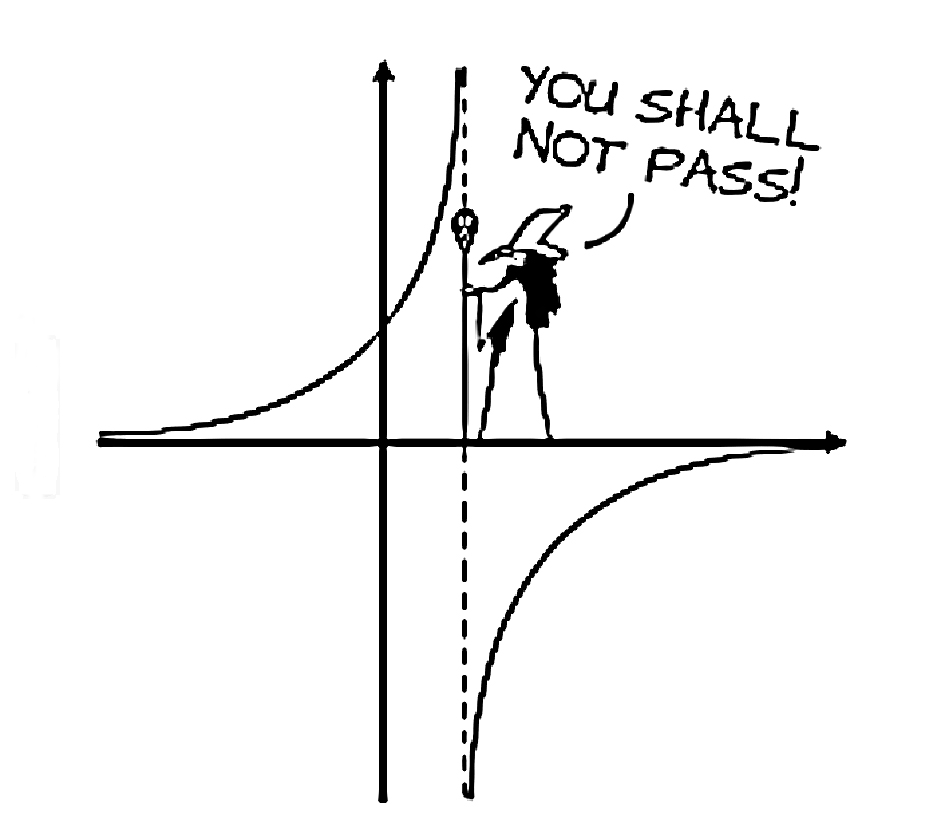
\includegraphics[width=8cm]{youshallnotpass}
%  \vfill
\end{center}
\vspace*{-3.5cm}
\begin{singlespace}
\subsection*{Doelstelling}
Je kan \hfill  {\scriptsize(LP 2006-059, LI 1.3, ET 14, 31, 32)}
\begin{itemize}
  \item rationale vergelijkingen oplossen, waarbij de graad van teller en noemer hoogstens gelijk is aan twee
  \item aan de hand van het functievoorschrift:
    \begin{itemize}
    \item een tabel,
    \item het domein,
    \item de nulwaarden,
    \item het tekenverloop
    \end{itemize}
    bepalen van rationale functies waarbij de graad van teller en noemer hoogstens gelijk is aan twee
  \item kunnen aan de hand van de grafiek:
    \begin{itemize}
    \item domein,
    \item bereik,
    \item nulwaarden,
    \item tekenverloop,
    \item stijgen/dalen,
    \item extrema
    \end{itemize}
    bepalen van rationale functies waarbij de graad van teller en noemer hoogstens gelijk is aan twee
  \item rationale ongelijkheden oplossen (eventueel met behulp van ICT), waarbij de graad van teller en noemer hoogstens gelijk is aan twee
  \item het asymptotische gedrag van een grafiek aflezen
  \item vraagstukken/problemen oplossen die aanleiding geven tot een rationale vergelijking, ongelijkheid of functie
\end{itemize}
\end{singlespace}


\thispagestyle{empty}
\newpage


\thispagestyle{empty}
\tableofcontents
\newpage


\pagenumbering{arabic}

\pagestyle{fancy}
\fancyhead[RO,LE]{Rationale functies}
\fancyhead[RE,LO]{}

\section{Rationale vergelijkingen}

\subsection{Definitie}

\begin{mdframed}
Een {\bf rationale vergelijking} is een vergelijking van de vorm
$$\dfrac{t(x)}{n(x)}=0$$
met $t(x)$ en $n(x)$ veeltermen.
\end{mdframed}

Het randgeval waarbij $q(x)=c$ met $c$ een constante $\in \mathbb{R}$ is dan ook een veeltermvergelijking. Veeltermvergelijkingen werden reeds in een vorig hoofdstuk besproken.

\paragraph{Voorbeeld}

We lossen de vergelijking
$$\dfrac{x^2-4}{x^2+2x}=0$$
op. Hierbij is de teller $t(x)=x^2-4$ en de noemer $n(x)=x^2+2x$.

\begin{align*}
  && \dfrac{x^2-4}{x^2+2x} &= 0\\
  \Leftrightarrow &&              x^2-4 &= 0 \cdot (x^2+2x) \\
  \Leftrightarrow &&              x^2-4 &= 0\\
  \Leftrightarrow &&              x = 2 &\vee x = -2
\end{align*}

Dat gaat vlot. Voordat we onze oplossingen in een oplossingenverzameling plaatsen, maken we nog eerst de proef en merken we dat het fout gaat voor $x=-2$ in de noemer! De enige geldige oplossing is dus
$$V=\{2\}$$

\subsection{Bestaansvoorwaarde}
Als we vergelijkingen oplossen, dan eisen we dat de gevonden oplossingen wel degelijk in de vergelijking ingevuld kunnen worden. Bij rationale vergelijkingen zullen we daarom eisen dat de noemer geen nul wordt. Deze eis is de {\bf bestaansvoorwaarde} of kort {\bf BV}.

We krijgen dus de eis:
$$ \text{BV: } n(x) \neq 0 $$

\subsection{Werkwijze: algebraïsch oplossen van rationale vergelijkingen}
\begin{enumerate}[(1)]
\item Je herleidt de gegeven vergelijking op nul.
\item Je stelt de bestaansvoorwaarde op.
\item Je stelt de teller gelijk aan nul en lost deze op.
\item Je schrijft de oplossingsverzameling $V$, hier komen alle oplossingen in als ze voldoen aan de bestaansvoorwaarde.
\end{enumerate}

\subsection{Oefeningen}

\begin{oefening} % voorbeeld oefeningen
Los op in $\mathbb{R}$:
\begin{exlist}{2}
\item $\dfrac{x-6}{x+4}=0$
\item $\dfrac{3}{x-2}=1$
\item $\dfrac{x}{x-5}+2=\dfrac{5}{x-5}$
\item $\dfrac{x-2}{x+2}=2+\dfrac{1}{x+2}$
\item $\dfrac{1}{x}+\dfrac{1}{x+1}=\dfrac{2}{x+2}$
\end{exlist}
\end{oefening}

\begin{oefening} % graad teller/noemer ten hoogste 2
Los op in $\mathbb{R}$:
\begin{exlist}{2}
  \item $\dfrac{x-1}{x+1}=3-\dfrac{2}{x+1}$
  \item $\dfrac{x+4}{x+2}=-x^2-2x+2$
  \item $\dfrac{x-3}{2(x-2)}+\dfrac{1}{x-3}=\dfrac{1}{(x-2)(x-3)}$
  \item $1+\dfrac{4}{x}=-\dfrac{4}{x^2}$
  \item $\dfrac{4x+9}{x+1}=\dfrac{4x+1}{x-1}$
  \item $\dfrac{3}{2x-5}=x$
  \item $\dfrac{3}{5-x}+\dfrac{2}{4-x}=\dfrac{5}{3-x}$
  \item $\dfrac{x-3}{x+2}=0$
  \item $\dfrac{2}{x-5}=1$
  \item $\dfrac{x}{x-5}+2=\dfrac{5}{x-5}$
  \item $\dfrac{x-1}{x+1}=3+\dfrac{1}{x+1}$
  \item $\dfrac{1}{x}+\dfrac{1}{x+1}=\dfrac{2}{x+2}$
  \item $\dfrac{1}{x+2}+\dfrac{4}{3x-4}=1$
  \item $\dfrac{x^2-1}{(x+1)^2}=0$
  \item $\dfrac{x+2}{x-7}+2=\dfrac{3x+1}{x-3}$
  \item $\dfrac{1}{x}-\dfrac{5}{2x-3}=\dfrac{x+1}{2x^2-3x}$
\end{exlist}
\end{oefening}

\begin{oefening} % hogere graads oefeningen
Los op in $\mathbb{R}$:\\
\begin{enumerate}[(a)]
  \itemsep.4em
  \item $\dfrac{7}{x+3} + x - \dfrac{6}{x} = \dfrac{4x-9}{x(x+3)} + 2$
\end{enumerate}
\end{oefening}

\begin{oefening}{\scriptsize\em IJkingsproef industrieel ingenieur, Ann De Bodt, Tanje Van Hecke}\\
Bepaal de weerstand $r$, uitgedrukt in $\Omega$, als je weet dat:
$$\dfrac{100}{4.7-r}=\dfrac{120}{\quad\dfrac{5.6r}{5.6+r}\quad}$$
Bereken de oplossing tot op 3 cijfers na het decimaal punt nauwkeurig uit!
Maak hier gebruik van een \zrm{ZRM}.
\begin{enumerate}[(A)]
  \itemsep.5em
  \item $r \approx 7.013\ \Omega$ en $r \approx -1.121\ \Omega$
  \item $r \approx 3.053\ \Omega$
  \item $r \approx 7.013\ \Omega$
  \item $r \approx 3.053\ \Omega$ en $r \approx -8.620\ \Omega$
\end{enumerate}
\end{oefening}

\subsection{Toepassingen}

\begin{oefening}
Een getal en zijn omgekeerde zijn samen $\frac{10}{3}$. Bepaal dit getal.
\end{oefening}

\begin{oefening}
Iemand wil 60 knikkers onder enkele kinderen verdelen. Waren er drie kinderen minder, dan kreeg elk kind 1 noot meer. Hoeveel kinderen waren er?
\end{oefening}

\begin{oefening}
Enkele personen verdelen 15000 euro. Indien er 5 personen minder geweest waren, dan zou elke persoon 150 euro meer gekregen hebben. Hoeveel personen zijn er?
\end{oefening}

\begin{oefening}
Een vrachtwagen moet 400 ton zand vervoeren en maakt daarvoor een aantal ritten, telkens volgeladen. Als de vrachtwagen 2 ton meer per rit kon laden, dan moet hij 10 ritten minder maken. Bepaal het laadvermogen van de oorspronkelijke vrachtwagen.
\end{oefening}

\begin{oefening}
Een getal en driemaal zijn omgekeerde zijn samen vier. Welk getal zoeken we? \hfill {\em (1 of 3)}
\end{oefening}

\begin{oefening}
De som van de omgekeerden van twee opeenvolgende gehele getallen is $\frac{9}{20}$. Bepaal die getallen. \hfill {\em (4 en 5)}
\end{oefening}

\begin{oefening}
Een leraar moet 200 overhoringen verbeteren. Per uur verbetert hij er 2 minder dan gepland en daarom moet hij 5 uur langer werken dan hij eerst gedacht had. Hoeveel overhoringen had hij er per uur willen verbeteren? \hfill {\em (10)}
\end{oefening}

\begin{oefening}
Een handelaar bestelt een aantal kristallen glazen en betaalt hiervoor 6000 euro. Bij aankomst blijken er 10 glazen meer te zijn dan hij besteld had. Daardoor daalt de prijs per stuk met 1 euro. Hoeveel glazen heeft de handelaar besteld en wat was de oorspronkelijke prijs per stuk? \hfill {\em (240 glazen en 25 euro per stuk)}
\end{oefening}

\begin{oefening}
Een knutselaar kocht voor 1200 euro verf. Als elke pot 20 euro meer zou kosten, dan had hij 5 potten minder kunnen kopen voor hetzelfde bedrag. Hoeveel potten verf kocht die knutselaar?
\end{oefening}

\pagebreak
\section{Rationale functies}

\subsection{Definities}

Wanneer we een functie $f(x)$ hebben waarbij er een breuk is met in de noemer een onbepaalde $x$, zullen we van een rationale functie spreken.

\paragraph*{Definitie}
\begin{mdframed}
Een {\bf rationale functie} is een reële functie met een voorschrift van de vorm

$$f(x)=\dfrac{t(x)}{n(x)}$$

waarbij $t(x)$ en $n(x)$ veeltermen zijn, en waarbij uiteraard de noemer niet de nulveelterm is.
\end{mdframed}

Wij bestuderen rationale functies waarbij de graad van teller en noemer $\leq 2$ is. In wat volgt zullen we vaak rekening moeten houden met de nulwaarden uit de noemer. Daarom geven we daar een naam aan.

\paragraph*{Definitie}
\begin{mdframed}
Een nulwaarde van de noemer, dus een $x$ zodat $n(x)=0$, noemen we een {\bf pool van de functie}, kortweg pool.
\end{mdframed}


In dit hoofdstuk zal steeds naar voor komen dat rationale functies een bepaalde waarde kunnen naderen. We definiëren daarom ook nog.

\paragraph*{Definitie}
\begin{mdframed}
Een rechte waarnaar een functie blijft naderen zonder deze ooit te snijden noemen we een {\bf asymptoot van de functie}, kortweg asymptoot.
\end{mdframed}

We spreken expliciet van naderen. Dit wordt soms verward met niet mogen snijden. Maar het is niet omdat een functie de asymptoot snijdt, dat de asymptoot de asymptoot niet meer is! De grafiek mag enkel de asymptoot niet snijden terwijl die ernaar nadert. Zo heeft onderstaande functie bijvoorbeeld een horizontale asymptoot $y=1$, terwijl de asymptoot de functie snijdt in $(5,1)$.

\begin{center}
  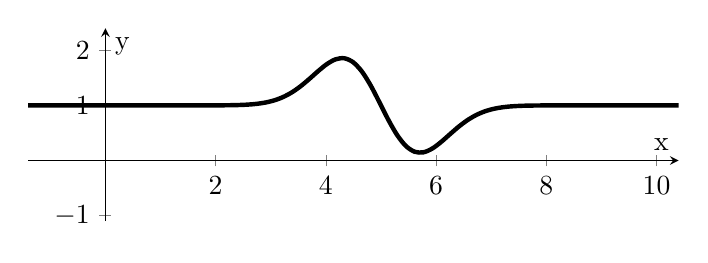
\begin{tikzpicture}
    \begin{axis}[
      scale=.7,
      x=1.0cm,y=1.0cm,
      axis lines=middle,
      xmin=-1.4,
      xmax=10.4,
      ymin=-1.1,
      ymax=2.4,
      xlabel={x},
      ylabel={y},
      samples=100]
      \addplot[line width=1.6pt,smooth,domain=-5.4:10.4] {-2*x*exp(-(x-5)^2)+10*exp(-(x-5)^2) + 1};
    \end{axis}
  \end{tikzpicture}
\end{center}

We zullen nu al grafisch asymptoten leren opsporen. Het correct wiskundig definiëren en algebraïsch bepalen van asymptoten zullen we pas in het hoofdstuk over {\em limieten} leren, zie later.

\subsection{Basisfunctie $y=\frac{1}{x}$}

De meest eenvoudige rationale functie is
$$f(x) = \dfrac{1}{x}$$

\paragraph{Grafiek:}\vspace*{-1cm}
\begin{center}
  \begin{tikzpicture}
    \begin{axis}[
      scale=.7,
      x=1.0cm,y=1.0cm,
      axis lines=middle,
      xmin=-9.4,
      xmax=12.4,
      ymin=-5.4,
      ymax=6.4,
      xlabel={x},
      ylabel={y},
%      xticklabels={-6,-5},
%      yticklabels={-1,0,1},
      samples=100]
      \addplot[line width=1.6pt,smooth,domain=-12.4:-0.1] (x,1/x);
      \addplot[line width=1.6pt,smooth,domain=0.1:12.4] (x,1/x);
    \end{axis}
  \end{tikzpicture}
\end{center}

Deze grafiek noemen we een {\bf hyperbool}.

\paragraph{Domein:}
0 heeft geen beeld, dus
$$\dom f = \mathbb{R}_0$$

\paragraph{Bereik:}
We merken dat $y=0$ ontbreekt als we de grafiek samendrukken op de $y$-as, dus
$$\ber f = \mathbb{R}_0$$
\paragraph{Nulwaarden:}
De $x$-as heeft geen snijpunten met de grafiek, dus
$$\mbox{nulp } f: \diagup$$

\paragraph{Asymptoten:}
De grafiek nadert zowel de $x$-as als de $y$-as. Dit zijn dus allebei asymptoten. De $x$-as noemen we dan een horizontale asymptoot (HA). De $y$-as noemen we dan een verticale asymptoot (VA). Dus
$$\text{HA}: y=0$$
$$\text{VA}: x=0$$

\subsection{Homografische functies $y=\frac{ax+b}{cx+d}$}

\paragraph*{Definitie}
\begin{mdframed}
Een {\bf homografische functie} is een functie van de vorm
$$f(x)=\dfrac{ax+b}{cx+d}$$
met $c\neq 0$ en $a\cdot d\neq b\cdot c$.
\end{mdframed}

\begin{oefening}
Zijn volgende functies homografisch?
\begin{exlist}{2}
  \item $f(x)=\dfrac{5x-3}{x-2}$
  \item $f(x)=\dfrac{4x-4}{x-1}$
  \item $f(x)=\dfrac{5}{x-3}$
  \item $f(x)=\dfrac{2x-4}{x-2}$
  \item $f(x)=\dfrac{x^2-4}{x+4}$
  \item $f(x)=\dfrac{4x^2-8}{2}$
  \item $f(x)=\dfrac{x^2-4}{x-4}$
  \item $f(x)=\dfrac{1+4x}{x}+\dfrac{3x-6}{x}$
  \item $f(x)=\dfrac{1+x^2}{\sqrt{x}+3}$
  \item $f(x)=\dfrac{3x^3-x^2-2}{x^4+x^3-x^2-1}$
\end{exlist}
\end{oefening}

\begin{oefening}
\begin{enumerate}[(a)]
  \item Zijn alle rationale functies homografische functies?
  \item Zijn alle homografische functies rationale functies?
\end{enumerate}
\end{oefening}

\subsubsection*{Bespreken van een homografische functie}

\paragraph{Voorbeeld} Beschouw de functie
$$f(x)=\dfrac{2x-4}{x+3}$$

\paragraph{Nulwaarden} We bepalen eerst van teller en noemer apart de
nulwaarden:
$$\text{nulw T: } x=2$$
$$\text{nulw N: } x=-3$$
We vinden dus alvast dat de functie één pool heeft, namelijk
$$\text{polen f: } -3$$
De nulwaarde van de functie is dan de nulwaarde van de teller, want de
nulwaarde van de teller komt er niet mee overeen. Dit zal bij de
``brave'' homografische functies steeds zo zijn. We krijgen dus
$$\text{nulw f: } x=2$$

\paragraph{Domein} Onze functie mag geen nul zijn in de noemer, we
moeten dus alle polen uit het domein halen, we krijgen
$$\dom f = \mathbb{R} \setminus \{-3\}$$

\paragraph{Asymptoten} Daar onze functie steeds dichter zal naderen
naar de pool, zonder deze echter te bereiken, bevind zich daar alvast
een verticale asymptoot, dus
$$\text{V.A.: } x=-3$$
Bij de ``brave'' homografische functies vinden we ook nog een
horizontale asymptoot, we kunnen daarvoor de coëfficiënt bij $x$ in de
teller delen door de coëfficiënt bij $x$ in de noemer, dus
$$\text{H.A.: } y=\dfrac{2\color{gray}x}{1\color{gray}x} \Rightarrow y=2$$

\paragraph{Bereik} Bij onze ``brave'' homografische functies zal de
functie nooit de horizontale asymptoot bereiken. We krijgen dus
$$\ber f = \mathbb{R} \setminus \{2\}$$

\paragraph{Tekenverloop} Een rationale functie kunnen we opsplitsen in
teller en noemer. We gebruik nu terug deze opsplitsing om het
tekenverloop te bepalen. Merk op dat we nu wel rekening moeten houden
met het niet mogen delen door nul. We krijgen volgend tekenschema

\begin{center}
  \begin{tabu} to\linewidth {X[3$c$]|*7{X[$c$]}}
    x                     & -\infty &   & -3 &   & 2 &   & +\infty\\
    \hline
    2x-4                  &    & - &    & - & 0 & + &   \\
    x+3                   &    & - &  0 & + &   & + &   \\
    \hline
    f(x)=\frac{2x-4}{x+3} &    & + &  | & - & 0 & + &
  \end{tabu}
\end{center}

\paragraph{Snijpunten} De snijpunten met de assen zijn eenvoudig te
bepalen, we hebben
$$\text{snijpt $x$-as: } (2,0)$$
$$\text{snijpt $y$-as: } (0,-\dfrac{4}{3})$$

\paragraph{Grafiek}
\begin{center}
  \begin{tikzpicture}
    \begin{axis}[
      scale=0.6,
      x=1.0cm,y=1.0cm,
      axis lines=middle,
      xmin=-14.3,
      xmax=12.3,
      ymin=-8.3,
      ymax=10.3,
      xtick={-14.0,-12.0,...,12.0},
      ytick={-8.0,-6.0,...,10.0},
      vasymptote=-3,
      hasymptote=2,
      ]
      \addplot[line width=1.8pt,smooth,samples=300,domain=-14.3:12.3, restrict y
      to domain=-10:11]
      {(2*x-4)/(x+3)};
      \begin{scriptsize}
        \draw (-10.,4.) node {$f$};
      \end{scriptsize}
    \end{axis}
  \end{tikzpicture}
\end{center}

\paragraph{Stijgen\&dalen en de extrema}
We zien op de grafiek dat onze functie enkel stijgt. Er zijn geen
extrema. Rekening houdend met de verticale asymptoot krijgen we
volgend schema

\begin{center}
  \begin{tabu} to\linewidth {X[3$c$]|*5{X[$c$]}}
    x                     & -\infty &   & -3 &   & +\infty\\
    \hline
    f(x)=\frac{2x-4}{x+3} &    & \nearrow &  | & \nearrow &
  \end{tabu}
\end{center}

\paragraph*{Homografische functies bespreken}
\begin{mdframed}
  \begin{itemize}
  \item Functievoorschrift: $f(x)=\dfrac{ax+b}{cx+d} \;.$
  \item polen f: $-\dfrac{d}{c}$
  \item $\dom f = \mathbb{R} \setminus \{\text{polen}\}$
  \item nulw f: $x_0=-\dfrac{b}{a}$
  \item V.A.: $x=$polen
  \item H.A.: $y=\dfrac{\text{coëff }x}{\text{coëff }x}$
  \item $\ber f = \mathbb{R} \setminus \{\text{H.A.}\}$
  \item t.v.: door splitsen in teller en noemer
  \item snijpunten bepalen
  \item Grafiek schetsen
  \item Stijgen\&dalen: a.d.h.v. de grafiek
  \end{itemize}
\end{mdframed}


\begin{oefening}
Bespreek volgende rationale functies waarbij teller en noemer van de eerste graad zijn (polen, domein, asymptoten, bereik, nulwaarden, snijpunten met de y-as, tekenschema, grafiek, stijgen/dalen/extrema):
\begin{exlist}{2}
  \item $f:y=\dfrac{2x+4}{x-1}$
  \item $f:y=\dfrac{2x+12}{x-4}$
  \item $f:y=\dfrac{4x+20}{4-x}$
  \item $f:y=\dfrac{3x+12}{2-x}$
  \item $f:y=\dfrac{10x+20}{5x-5}$
  \item $f:y=\dfrac{5x+30}{6-x}$
  \item $f:y=\dfrac{3x-27}{3x+9}$
\end{exlist}
\end{oefening}

\subsection{Rationale funties $y=\frac{t(x)}{n(x)}$}

\begin{oefening}
Bespreek volgende rationale functies waarbij teller en noemer van de tweede graad zijn (polen, domein, asymptoten, bereik, nulwaarden, snijpunten met de y-as, tekenschema, grafiek, stijgen/dalen/extrema):
\begin{multicols}{2}
\begin{enumerate}[(a)]
  \itemsep0.6em
  \item $f:y=\dfrac{x^2-1}{x^2-4}$
  \item $f:y=\dfrac{x^2-2x-24}{x^2-9}$
  \item $f:y=\dfrac{x^2+2x-15}{x^2-4}$
  \item $f:y=\dfrac{2x^2+2x+1}{x^2-1}$
  \item $f:y=\dfrac{x+1}{(x-1)^2}$
  \item $f:y=\dfrac{x^2}{x^2+2x+1}$
  \item $f:y=\dfrac{x^2}{(x+1)^2}$
  \item $f:y=\dfrac{x-1}{x^2}$
  \item $f:y=\dfrac{x^2-4}{x^2-1}$
  \item $f:y=\dfrac{x^2-1}{x+1}$
\end{enumerate}
\end{multicols}
\end{oefening}

\begin{oefening}*
Bespreek volgende rationale functies (polen, domein, asymptoten, bereik, nulwaarden, snijpunten met de y-as, tekenschema, grafiek, stijgen/dalen/extrema):\\
\begin{enumerate}[(a)]
  \itemsep0.6em
  \item $f:y=\dfrac{x^2-1}{x+1}$
\end{enumerate}
\end{oefening}

\subsection{Toepassingen}


\begin{oefening}
De grootte van een konijnenpopulatie wordt gegeven door
$$f(x)=\dfrac{150x+90}{x+3}\;.$$
De functie $f(x)$ stelt het aantal konijnen voor en $x$ de tijd in maanden.
\begin{enumerate}[(a)]
  \item Bepaal het praktische domein.
  \item Hoeveel konijnen zijn er op tijdstip 0?
  \item Na hoeveel maand zijn er meer dan 100 konijnen?
\end{enumerate}
\end{oefening}

\begin{oefening}
Het lokaal van de jeugdbeweging is aan een grondige opknapbeurt toe. {\em ''Vele handen maken licht werk''} redeneert men. De functie
$$d(x)=\dfrac{3x+25}{x}$$
geeft het aantal dagen nodig voor de opknapbeurt, in functie van het aantal vrijwilligers $x$.
\begin{enumerate}[(a)]
  \item Bepaal het praktische domein.
  \item Hoeveel vrijwilligers heeft men minimaal nodig om de klus in 4 dagen te klaren?
\end{enumerate}
\end{oefening}

\begin{oefening}
Een schoonmaakbedrijf hanteert de formule $k(x)=9+\dfrac{40}{x}$ voor het schoonmaken van gebouwen. Hierin is $k(x)$ het bedrag in euro dat per jaar per $\m^2$ moet worden betaald en $x$ de oppervlakte in $100 \m^2$.
\begin{enumerate}[(a)]
  \item Een vloeroppervlak is $2000 \m^2$. Hoeveel moet er per jaar voor het schoonmaken betaald worden?
  \item Kasper zou zijn studentenkot van 8 bij 6 meter door het bedrijf willen laten onderhouden. Hoeveel kost hem dat per jaar?
  \item Firma Xanders betaalt jaarlijks 9.16 euro per $\m^2$ voor het schoonmaken van zijn gebouw. Hoe groot is de oppervlakte van dit gebouw?
\end{enumerate}
\end{oefening}

\begin{oefening}
De populatie vossen in een bepaald gebied was nagenoeg constant. Doch door een tot nu toe onbekende oorzaak werd dit evenwicht verstoord. De hoeveelheid vossen in functie van de tijd wordt nu benaderd door de functie
$$v(t)=\dfrac{3t^2-12t+13}{t^2-4t+5}\;.$$
Hierbij is
\begin{itemize}
  \item v = aantal vossen, uitgedrukt in duizendtallen
  \item t = tijd in jaren
  \item t = 0 komt overeen met januari 2010
\end{itemize}
Van wanneer tot wanneer waren er minder dan 2000 vossen in het gebied?
\end{oefening}

\begin{oefening}
De temperatuur in een koele berging wordt gegeven door de volgende functie:
$$T(t)=\dfrac{3t^2-6t+3}{t^2-2t+2}\;.$$
Hierbij is
\begin{itemize}
  \item T = de temperatuur in graden Celsius
  \item t = tijd in uren
  \item t = 0 komt overeen met 3 uur 's nachts.
\end{itemize}
Als de temperatuur lager wordt dan 1 $^\circ$C is er gevaar voor schade aan het voedsel. Hoe lang bevond de temperatuur zich onder 1 $^\circ$C? Van wanneer tot wanneer?
\end{oefening}

\pagebreak
\section{Rationale ongelijkheden}

\begin{oefening}
Los op in $\mathbb{R}$. Met andere woorden bepaal $V$.
\begin{multicols}{2}
\begin{enumerate}[(a)]
  \itemsep.5em
  \item $x-\dfrac{2}{x}>1$
  \item $\dfrac{x-1}{x+2}\leq\dfrac{x+2}{x-4}$
  \item $\dfrac{4x+9}{x+1}\geq\dfrac{4x+1}{x-1}$
  \item $\dfrac{x+4}{x+2}\geq -x^2-2x+2$
  \item $\dfrac{x}{x+3}\geq\dfrac{10}{(x+3)^2}$
  \item $\dfrac{x^2+3x+2}{x^2-16}\geq0$
  \item $\dfrac{(-2x-10)(3-x)}{(x^2+5)(x-2)^2}<0$
  \item $\dfrac{x+1}{x-5}\leq 0$
  \item $\dfrac{x^2+4x+3}{x-1}>0$
  \item $\dfrac{x^2-16}{(x-1)^2}<0$
  \item $\dfrac{3x+1}{x+4}\geq 1$
  \item $\dfrac{x-8}{x}\leq 3-x$
\end{enumerate}
\end{multicols}
\end{oefening}

\begin{oefening}{\scriptsize\em IJkingsproef hoger onderwijs, Ann De Bodt, Tanje Van Hecke}\\
Los op naar $x\in\mathbb{R}$ : $\dfrac{1}{|x-2|}\leq 1$\\
\begin{enumerate}[(A)]
  \itemsep.5em
  \item $x\in]-\infty, 1]$
  \item $x\in]-\infty, 1]\cup[3,+\infty[$
  \item $x\in[3,+\infty[$
  \item $x\in]3,+\infty[$
\end{enumerate}
\end{oefening}

\begin{oefening}{\scriptsize\em IJkingsproef hoger onderwijs, Ann De Bodt, Tanje Van Hecke}\\
Bepaal de oplossingsverzameling van $\dfrac{1}{x} - 4 \geq 1$\\
\begin{enumerate}[(A)]
  \itemsep.5em
  \item $]-\infty, 5]$
  \item $[0, \dfrac{1}{5}]$
  \item $]0, \dfrac{1}{5}]$
  \item $]-\infty, \dfrac{1}{5}]$
\end{enumerate}
\end{oefening}

\needspace{3cm}
\subsection{Toepassingen}

\begin{oefening}
De grootte van een konijnenpopulatie wordt gegeven door
$$f(x)=\dfrac{150x+90}{x+3}\;.$$
De functie $f(x)$ stelt het aantal konijnen voor en $x$ de tijd in maanden.
\begin{enumerate}[(a)]
  \item Bepaal het praktische domein.
  \item Hoeveel konijnen zijn er op tijdstip 0?
  \item Na hoeveel maand zijn er meer dan 100 konijnen?
\end{enumerate}
\end{oefening}

\begin{oefening}
Het lokaal van de jeugdbeweging is aan een grondige opknapbeurt toe. {\em ''Vele handen maken licht werk''} redeneert men. De functie
$$d(x)=\dfrac{3x+25}{x}$$
geeft het aantal dagen nodig voor de opknapbeurt, in functie van het aantal vrijwilligers $x$.
\begin{enumerate}[(a)]
  \item Bepaal het praktische domein.
  \item Hoeveel vrijwilligers heeft men minimaal nodig om de klus in 4 dagen te klaren?
\end{enumerate}
\end{oefening}

\begin{oefening}
Een schoonmaakbedrijf hanteert de formule $k(x)=9+\dfrac{40}{x}$ voor het schoonmaken van gebouwen. Hierin is $k(x)$ het bedrag in euro dat per jaar per m$^2$ moet worden betaald en $x$ de oppervlakte in 100 m$^2$.
\begin{enumerate}[(a)]
  \item Een vloeroppervlak is 2000 m$^2$. Hoeveel moet er per jaar voor het schoonmaken betaald worden?
  \item Kasper zou zijn studentenkot van 8 bij 6 meter door het bedrijf willen laten onderhouden. Hoeveel kost hem dat per jaar?
  \item Firma Xanders betaalt jaarlijks 9.16 euro per m$^2$ voor het schoonmaken van zijn gebouw. Hoe groot is de oppervlakte van dit gebouw?
\end{enumerate}
\end{oefening}

\begin{oefening}
De populatie vossen in een bepaald gebied was nagenoeg constant. Doch door een tot nu toe onbekende oorzaak werd dit evenwicht verstoord. De hoeveelheid vossen in functie van de tijd wordt nu benaderd door de functie
$$v(t)=\dfrac{3t^2-12t+13}{t^2-4t+5}\;.$$
Hierbij is
\begin{itemize}
  \item $v$ = aantal vossen, uitgedrukt in duizendtallen
  \item $t$ = tijd in jaren
  \item $t = 0$ komt overeen met januari $2010$
\end{itemize}
Van wanneer tot wanneer waren er minder dan $2000$ vossen in het gebied?
\end{oefening}

\begin{oefening}
De temperatuur in een koele berging wordt gegeven door de volgende functie:
$$T(t)=\dfrac{3t^2-6t+3}{t^2-2t+2}\;.$$
Hierbij is
\begin{itemize}
  \item $T$ = de temperatuur in graden Celsius ($\grC$)
  \item $t$ = tijd in uren
  \item $t = 0$ komt overeen met 3 uur 's nachts.
\end{itemize}
Als de temperatuur lager wordt dan $1 \grC$ is er gevaar voor schade aan het voedsel. Hoe lang bevond de temperatuur zich onder $1 \grC$? Van wanneer tot wanneer?
\end{oefening}

\end{document}



